\subsection{斯特林展开}

设 \(x\) 与 \(y\) 是两个不在实负半轴上的复数；由 VII, p.~315 的公式 (3) ，并依照 VII, p.~316 关于对数的约定，\(\log \Gamma(x) - \log \Gamma(y)\) 模 \(2\pi i\) 同余于表达式

\[
(x - y) \log n + \sum_ {k = 0} ^ {n} \Big (\log (y + k) - \log (x + k) \Big).\tag{15}
\]

令 \(f(t) = \log(y + t) - \log(x + t)\) ；对函数 f 应用欧拉–麦克劳林求和公式（VI, p.~288）：

\[
\begin{array}{l} f (0) + f (1) + \dots + f (n) = \int_ {0} ^ {n + 1} f (t) d t - \frac {1}{2} \big (f (n + 1) - f (0) \big) \\ \qquad + \sum_ {k = 1} ^ {p} \frac {b _ {2 k}}{(2 k) !} \big (f ^ {(2 k - 1)} (n + 1) - f ^ {(2 k - 1)} (0) \big) + T _ {p} (n) \end{array}
\]

其中

\[
\left| \mathrm{T} _ {p} (n) \right| \leqslant \frac {4 e ^ {2 \pi}}{(2 \pi) ^ {2 p + 1}} \int_ {0} ^ {n + 1} \left| f ^ {(2 p + 1)} (u) \right| d u.\tag{16}
\]

由于

\[
f ^ {(m)} (t) = (- 1) ^ {m - 1} (m - 1)! \left(\frac {1}{(y + t) ^ {m}} - \frac {1}{(x + t) ^ {m}}\right),
\]

\(f^{(2k - 1)}(n + 1)\) 当 \(n\) 趋于 \(+\infty\) 时趋于 0 （对一切 \(k \geqslant 1\) ）；对

\[
f (n + 1) = \log \left(1 + \frac {y}{n + 1}\right) - \log \left(1 + \frac {x}{n + 1}\right).
\]

此外，有

\[
\int_ {0} ^ {n + 1} \log (x + t) d t = (x + n + 1) (\log (x + n + 1) - 1) - x (\log x - 1);
\]

当 n 趋于 \(+\infty\) 时，有渐近展开

\[
(x + n) \bigl (\log (x + n) - 1 \bigr) = n \log n - n + x \log n + O \left(\frac {1}{n}\right).
\]

把这些结果代入表达式 (15) ，最终可以看出，当 n 趋于 \(+\infty\) 时，\(\mathrm{T}_{p}(n)\) 有极限 \(\mathrm{R}_{p}(x, y)\) ，并且可以写

\[
\log \Gamma (x) - g (x) \equiv \log \Gamma (y) - g (y) + \mathrm{R} _ {p} (x, y)\tag{mod.  \( 2\pi i \)}
\]

其中令

\[
g (x) = x \log x - x - \frac {1}{2} \log x + \sum_ {k = 1} ^ {p} \frac {b _ {2 k}}{2 k (2 k - 1)} \frac {1}{x ^ {2 k - 1}}.\tag{17}
\]

现在我们借助 (16) 来估计 \(\mathrm{R}_{p}(x,y)\) 的一个上界，假设 x 与 y 都属于 C 中的子集 \(H_{A}\) ——由关系式`` \(\mathcal{R}(z)\geqslant A\) 或 \(|\mathcal{I}(z)|\geqslant A\) ''所定义——其中 A 是任意数 \textgreater0 （图~2）。为此我们注意到，若 \(x=s+it\) 且 s\textgreater A ，则有 \(|x+u|\geqslant A+u\) （对每个 u\textgreater0 ），因而

\[
\int_ {0} ^ {n + 1} \frac {d u}{| x + u | ^ {2 p + 1}} \leqslant \int_ {0} ^ {\infty} \frac {d u}{(\mathrm{A} + u) ^ {2 p + 1}} = \frac {1}{2 p \mathrm{A} ^ {2 p}}.
\]

同样，若 \(|t| \geqslant A\) ，则有 \(|x + u| = |s + u + it| \geqslant \sqrt{A^2 + (s + u)^2}\) （对一切实数 \(u\) ），由此得

\[
\int_ {0} ^ {n + 1} \frac {d u}{| x + u | ^ {2 p + 1}} \leqslant \int_ {- \infty} ^ {+ \infty} \frac {d u}{(\mathrm{A} ^ {2} + u ^ {2}) ^ {p + 1 / 2}} = \frac {2}{\mathrm{A} ^ {2 p}} \int_ {0} ^ {\infty} \frac {d v}{(1 + v ^ {2}) ^ {p + 1 / 2}}.
\]

于是可以看出，当 x 与 y 属于 \(H_{A}\) 时，有

\[
\left| \mathrm{R} _ {p} (x, y) \right| \leqslant \frac {\mathrm{C} _ {p}}{\mathrm{A} ^ {2 p}}
\]

\pandocbounded{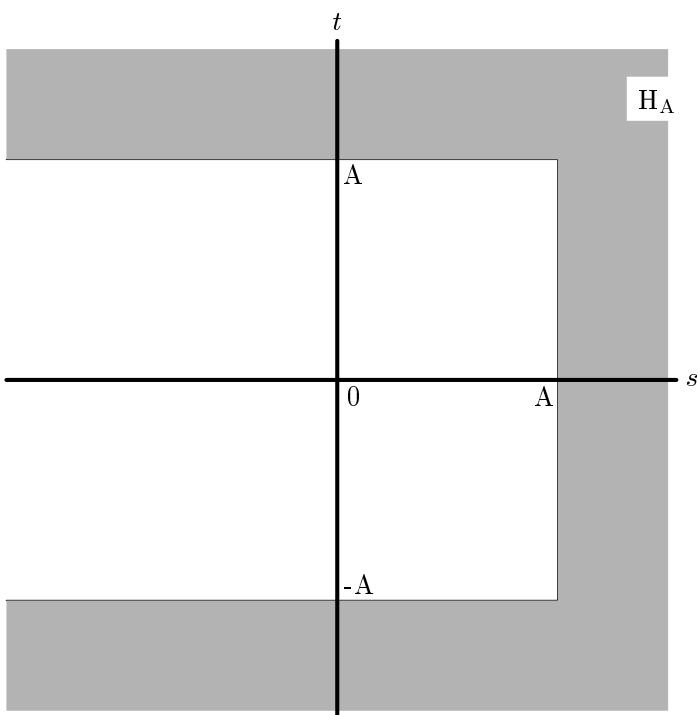
\includegraphics[keepaspectratio]{images/part002_194eed20.jpg}}\\
图 2

其中 \(C_{p}\) 仅依赖于 p。现设 F 是以诸集 \(H_{A}\) 为基的滤子；柯西准则表明，沿滤子 F ，函数 \(\log \Gamma(z) - g(z)\) 有一个有限极限 \(\delta\) （模 \(2\pi i\) ） ，并且，若令 \(\omega(z) = \max(\mathcal{R}(z), |\mathcal{I}(z)|)\) ，则有

\[
\log \Gamma (z) - g (z) - \delta \equiv O \left(\frac {1}{(\omega (z)) ^ {2 p}}\right) \pmod {2 \pi i}.\tag{18}
\]

对实数 \(x\) 且 \(> 0\) ，有 \(\Gamma(x) > 0\) ，且 \(g(x)\) 是实数，故可以设 \(\delta\) 是实数，并有

\[
\log \Gamma (x) = g (x) + \delta + O \left(\frac {1}{x ^ {2 p}}\right).
\]

现在来确定常数 \(\delta\) 的值；把 VII, p.~318 的 prop. 2 应用于 p = 2 ，则当实数 x 趋于 \(+\infty\) 时，有

\[
\begin{array}{c} \frac {x - 1}{2} \log \frac {x}{2} - \frac {x}{2} + \frac {x}{2} \log \frac {x + 1}{2} - \frac {x + 1}{2} + 2 \delta \\ = x \log x - x - \frac {1}{2} \log x + (\frac {1}{2} - x) \log 2 + \frac {1}{2} \log 2 \pi + \delta + o (1) \end{array}
\]

由此容易推出 \(\delta = \frac{1}{2}\log 2\pi\) 。最后有下列结果：

命题 4. 沿滤子 \(\mathfrak{F}\) ，有（对每个整数 \(p \geqslant 1\) ）渐近展开

\[
\begin{array}{l} \log \Gamma (z) \equiv z \log z - z - \frac {1}{2} \log z + \frac {1}{2} \log 2 \pi \\ \quad + \sum_ {k = 1} ^ {p} \frac {b _ {2 k}}{2 k (2 k - 1)} \frac {1}{z ^ {2 k - 1}} + O \left(\frac {1}{(\omega (z)) ^ {2 p}}\right) \pmod {2 \pi i} \end{array}\tag{19}
\]

（斯特林展开）。

推论. 沿滤子 F ，有

\[
\Gamma (z) \sim \sqrt {2 \pi} \exp (z \log z - z - \frac {1}{2} \log z).\tag{20}
\]

特别地，当实数 \(x\) 趋于 \(+\infty\) 时，公式 (20) 可以写成

\[
\Gamma (x) \sim \sqrt {2 \pi} x ^ {x - 1 / 2} e ^ {- x},\tag{21}
\]

于是，当整数 n 趋于 \(+\infty\) 时，

\[
n! \sim \sqrt {2 \pi} n ^ {n + 1 / 2} e ^ {- n}
\]

（cf.~V, p.~244）。

由此可以导出许多公式。例如，对每个复数 \(\alpha\) 与每个整数 n ，当 n 趋于 \(+\infty\) 时，有

\[
\frac {\Gamma (n + \alpha)}{\Gamma (n)} \sim n ^ {\alpha} \quad (= e ^ {\alpha \log n}).\tag{22}
\]

同样，对每个不是整数 \(\leqslant 0\) 的复数 a ，有

\[
a (a + 1) (a + 2) \dots (a + n) = \frac {\Gamma (n + a + 1)}{\Gamma (a)} \sim \frac {\sqrt {2 \pi}}{\Gamma (a)} n ^ {n + a + 1 / 2} e ^ {- n}\tag{23}
\]

而对每个不是整数 \(\geqslant 0\) 的复数 a ，有

\[
\binom {a} {n} = \frac {(- 1) ^ {n}}{\Gamma (- a)}   \frac {\Gamma (n - a)}{\Gamma (n + 1)} \sim \frac {(- 1) ^ {n}}{\Gamma (- a)}   n ^ {- a - 1}.\tag{24}
\]

最后，对每个实常数 \(k > 1\) ，有

\[
\binom {k n} {n} = \frac {\Gamma (k n + 1)}{\Gamma (n + 1)   \Gamma ((k - 1) n + 1)} \sim \sqrt {\frac {k}{2 \pi (k - 1) n}} \left(\frac {k ^ {k}}{(k - 1) ^ {k - 1}}\right) ^ {n}.\tag{25}
\]

同样的论证导出下面类似的命题：

命题 5. 沿滤子 \(\mathfrak{F}\) ，有（对每个整数 \(p \geqslant 1\) ）渐近展开

\[
\frac {\Gamma^ {\prime} (z)}{\Gamma (z)} = \log z - \frac {1}{2 z} - \sum_ {k = 1} ^ {p} \frac {b _ {2 k}}{2 k} \frac {1}{z ^ {2 k}} + O \left(\frac {1}{(\omega (z)) ^ {2 p + 1}}\right).\tag{26}
\]

这里不用 VII, p.~318 的 prop. 2 ，而使用公式

\[
\int_ {x} ^ {x + 1} \frac {\Gamma^ {\prime} (t)}{\Gamma (t)} d t = \log \Gamma (x + 1) - \log \Gamma (x) = \log x
\]

来确定常数。

\setcounter{exercisegroup}{0}
\refstepcounter{exercisegroup}
